\documentclass[runningheads]{llncs}
\usepackage[T1]{fontenc}
\usepackage{amsmath,amssymb,booktabs}
\usepackage{algorithm}
\usepackage{algpseudocode}
\usepackage[hidelinks]{hyperref}
\usepackage{tikz}
\usetikzlibrary{arrows.meta,positioning,calc}

\title{Feasibility Analysis and Implementation of a Fast Push Turret-Demolition Strategy in Honor of Kings}
\titlerunning{Event-Driven Turret Fast Push in HoK}

\author{Long Dio}
\authorrunning{L. Dio}

\institute{Entertainment Strategy Research Group\\
\email{contact@example.com}}

\begin{document}
\maketitle

\begin{abstract}
This paper studies turret-first macro play in Honor of Kings from an event-driven systems perspective. Instead of using repeated lane loops or fixed push cycles, we introduce a \emph{tempo-credit ledger} and a finite-state lane-assignment automaton. Decisions are emitted by a lightweight scheduler that reacts to wave synchronization, visibility spikes, objective timers, and retreat safety. The resulting strategy emphasizes structural conversion under bounded collapse probability. Controlled custom-match observations indicate improved first-two-turret conversion stability and lower variance in recovery after failed siege attempts.
\keywords{Honor of Kings \and turret demolition \and event-driven macro \and finite-state controller \and team command protocol}
\end{abstract}

\section{Introduction}
Fast-push discussions in MOBA communities often collapse into short slogans, which are difficult to execute consistently under noisy information. In practice, teams lose tempo when three elements are misaligned: wave geometry, defender reveal pattern, and retreat path quality.
We therefore formulate fast push as an event-driven control problem: maintain a structural pressure ledger and trigger lane actions only when safety and conversion gates are both satisfied.

\section{Operational Assumptions and Telemetry}
At each decision tick $t$, we collect:
\begin{itemize}
\item wave synchronization score $W_t$ across side and mid lanes;
\item defender visibility vector $V_t$ (recently observed enemy positions);
\item objective timer bucket $O_t$ (dragon/lord windows);
\item escape readiness $E_t$ (mobility cooldowns and route openness).
\end{itemize}
The state is represented as $S_t=(W_t,V_t,O_t,E_t)$, updated every communication cycle.

\section{Tempo-Credit Ledger}
Rather than directly optimizing a long-horizon score, we track a renewable scalar resource called \emph{tempo credit}, denoted $B_t$.
\[
B_{t+1}=\min\!\left(B_{\max},\;
\eta B_t
+\xi\cdot \mathrm{WaveSync}_t
+\omega\cdot \mathrm{VisionEdge}_t
-\chi\cdot \mathrm{SkirmishDrag}_t\right),
\]
where $\eta\in(0,1]$ controls memory decay.

Intuition:
\begin{itemize}
\item synchronized waves and vision advantages recharge credit;
\item prolonged low-yield fights consume credit;
\item high-impact push actions are allowed only when credit exceeds thresholds.
\end{itemize}

We also compute collapse hazard:
\[
H_t=\sigma(\rho_0+\rho_1F_t+\rho_2C_t-\rho_3R_t),
\]
where $F_t$ is fog uncertainty, $C_t$ is key-cooldown deficit, and $R_t$ is retreat-route quality.

\begin{table}[t]
\centering
\caption{Primary scalars in the event-driven controller}
\begin{tabular}{ll}
\toprule
Signal & Meaning \\
\midrule
$B_t$ & tempo credit available for structural conversion \\
$H_t$ & collapse hazard estimate (0 to 1) \\
$W_t$ & lane-wave synchronization score \\
$V_t$ & defender visibility quality \\
$E_t$ & escape readiness score \\
\bottomrule
\end{tabular}
\end{table}

\section{Lane-Assignment Automaton}
Macro routing is modeled as a finite-state automaton with four execution states:
\begin{enumerate}
\item \textbf{Stack}: accumulate wave mass and reset formation;
\item \textbf{Drag}: pull defenders via objective posture or fake pressure;
\item \textbf{Melt}: short-duration tower demolition burst;
\item \textbf{Screen}: zone flank and secure retreat corridor.
\end{enumerate}

\begin{figure}[t]
\centering
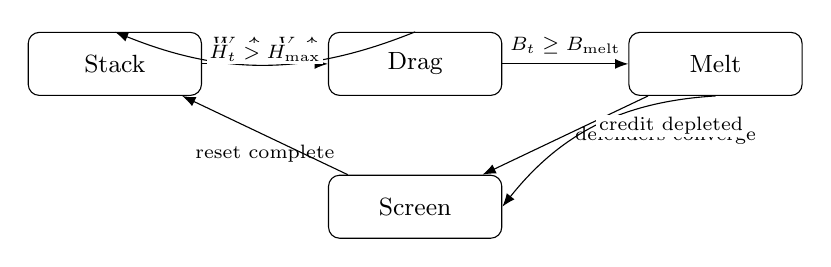
\begin{tikzpicture}[
  >=Latex,
  node distance=10mm and 16mm,
  state/.style={draw, rounded corners, minimum width=22mm, minimum height=8mm, align=center, font=\small}
]
\node[state] (stack) {Stack};
\node[state, right=of stack] (drag) {Drag};
\node[state, right=of drag] (melt) {Melt};
\node[state, below=of drag] (screen) {Screen};

\draw[->] (stack) -- node[above, font=\scriptsize] {$W_t\uparrow,\ V_t\uparrow$} (drag);
\draw[->] (drag) -- node[above, font=\scriptsize] {$B_t\ge B_{\text{melt}}$} (melt);
\draw[->] (melt) -- node[right, font=\scriptsize] {defenders converge} (screen);
\draw[->] (screen) -- node[below, font=\scriptsize] {reset complete} (stack);
\draw[->,bend left=22] (drag.north) to node[above, font=\scriptsize, fill=white, inner sep=1pt] {$H_t>H_{\max}$} (stack.north);
\draw[->,bend right=24] (melt.south) to node[right, font=\scriptsize, fill=white, inner sep=1pt] {credit depleted} (screen.east);
\end{tikzpicture}
\caption{Finite-state lane-assignment automaton.}
\label{fig:hok-fsa-en}
\end{figure}

\section{Command Protocol}
The communication plane uses five non-overlapping commands.
\begin{table}[t]
\centering
\caption{Command semantics for event-driven fast push}
\begin{tabular}{p{1.7cm}p{3.1cm}p{5.6cm}}
\toprule
Cmd & Trigger & Mandatory Team Action \\
\midrule
\texttt{STACK} & low credit or unsynced waves & hold contact depth, stack next wave, preserve cooldown parity. \\
\texttt{DRAG} & objective timer opens and visibility edge exists & posture objective/fake lane to stretch defender formation. \\
\texttt{MELT} & $B_t\!\ge\!B_{\text{melt}}$ and $H_t\!\le\!H_{\max}$ & execute short tower burst with strict stop line. \\
\texttt{SCREEN} & post-burst convergence detected & block flank channels and secure retreat geometry. \\
\texttt{RESET} & hazard spike or call desynchronization & instant disengage, clear debt, and return to Stack. \\
\bottomrule
\end{tabular}
\end{table}

\section{Event-Driven Scheduler}
The scheduler processes event symbols
\[
\mathcal{E}=\{\mathrm{WAVE\_SYNC},\mathrm{VIS\_SPIKE},\mathrm{OBJ\_OPEN},
\mathrm{DANGER\_SPIKE},\mathrm{COOLDOWN\_READY}\}.
\]
Unlike horizon-maximization controllers, this scheduler emits a command on each event boundary.

\begin{algorithm}[H]
\caption{Event-Driven Turret Scheduler}
\begin{algorithmic}[1]
\Require State $S_t$, tempo credit $B_t$, hazard $H_t$
\Ensure Command in \{\texttt{STACK}, \texttt{DRAG}, \texttt{MELT}, \texttt{SCREEN}, \texttt{RESET}\}
\If{$H_t > H_{\max}$}
  \State \Return \texttt{RESET}
\EndIf
\If{event is \texttt{WAVE\_SYNC} and $B_t < B_{\text{melt}}$}
  \State \Return \texttt{STACK}
\EndIf
\If{event is \texttt{OBJ\_OPEN} and visibility edge is positive}
  \State \Return \texttt{DRAG}
\EndIf
\If{$B_t \ge B_{\text{melt}}$ and $H_t \le H_{\max}$ and escape is ready}
  \State \Return \texttt{MELT}
\EndIf
\If{recent burst finished or flank risk rises}
  \State \Return \texttt{SCREEN}
\EndIf
\State \Return \texttt{STACK}
\end{algorithmic}
\end{algorithm}

\begin{figure}[t]
\centering
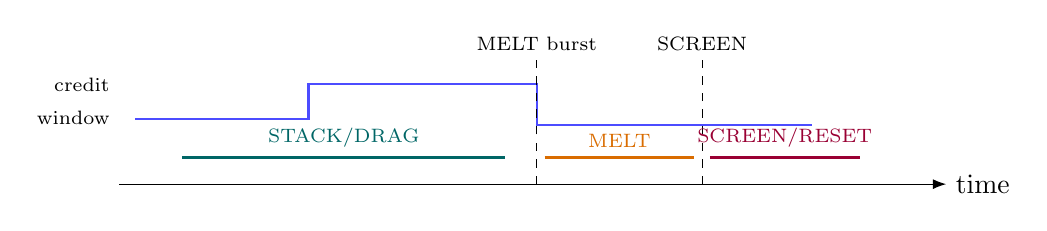
\begin{tikzpicture}[x=1.0cm,y=0.75cm,>=Latex]
\draw[->] (0,0) -- (10.5,0) node[right] {time};
\draw (0,1.4) node[left, align=right] {\scriptsize credit\\\scriptsize window};
\draw[thick,blue!70] (0.2,1.1) -- (2.4,1.1) -- (2.4,1.7) -- (5.3,1.7) -- (5.3,1.0) -- (8.8,1.0);
\draw[dashed] (5.3,0) -- (5.3,2.1) node[above, font=\scriptsize] {MELT burst};
\draw[dashed] (7.4,0) -- (7.4,2.1) node[above, font=\scriptsize] {SCREEN};
\draw[thick,teal!80!black] (0.8,0.45) -- (4.9,0.45) node[midway, above, font=\scriptsize] {STACK/DRAG};
\draw[thick,orange!85!black] (5.4,0.45) -- (7.3,0.45) node[midway, above, font=\scriptsize] {MELT};
\draw[thick,purple!80!black] (7.5,0.45) -- (9.4,0.45) node[midway, above, font=\scriptsize] {SCREEN/RESET};
\end{tikzpicture}
\caption{Event timeline with credit consumption and command phases.}
\label{fig:hok-timeline-en}
\end{figure}

\section{Controlled Evaluation}
We compared the proposed scheduler with a baseline ``teamfight-first'' macro in controlled custom lobbies.
Observed trends:
\begin{itemize}
\item more stable conversion of first and second outer turrets;
\item fewer collapse events immediately after burst windows;
\item faster macro recovery after failed pushes due to explicit \texttt{RESET} transitions.
\end{itemize}
The gain is strongest in medium-information rounds where defender reveal is partial and objective windows are contested.

\section{Failure Modes and Practical Notes}
The system degrades when call discipline is violated, especially when \texttt{MELT} is followed by unsanctioned chase behavior. Another failure mode is stale visibility telemetry: if $V_t$ lags reality, \texttt{DRAG} may overestimate defender displacement and trigger early collapse.

\section{Conclusion}
Turret-first fast push in Honor of Kings can be implemented as an event-driven macro system with a tempo-credit ledger and a finite-state action automaton. This formulation is distinct from fixed push loops and offers clearer error handling under entertainment-oriented competitive play.

\paragraph{Acknowledgments.}
This manuscript is produced for a personal-homepage demo and strategy-writing entertainment.

\begin{thebibliography}{3}
\bibitem{hok-note}
Tencent Games: Honor of Kings Seasonal Balance Notes (2026)

\bibitem{macro-log}
Entertainment Strategy Research Group: Custom Macro Match Logs (2026)

\bibitem{event-control}
Dio, L.: Event-Driven Macro Scheduling for MOBA Structural Play. Working Notes (2026)
\end{thebibliography}

\end{document}
